%
\documentclass{llncs}

\usepackage{url}
\usepackage{graphicx}
\usepackage[T1]{fontenc}
\usepackage[hidelinks]{hyperref}
\usepackage{pdfpages}
\usepackage{relsize}
\usepackage{tcolorbox}

\usepackage{svg}
\newcommand{\orcid}[1]{\href{https://orcid.org/#1}{\includesvg[height = 2ex]{svg-inkscape/ORCID_iD}}}

\newcommand{\ie}{\textit{, ie.\ }}

\def\codesize{\smaller}
\def\<#1>{\codeid{#1}}
\newcommand{\codeid}[1]{\ifmmode{\mbox{\codesize\ttfamily{#1}}}\else{\codesize\ttfamily #1}\fi}

\usepackage{listings, xcolor}

\renewcommand{\UrlFont}{\ttfamily\codesize}

\definecolor{verylightgray}{rgb}{.97,.97,.97}

\lstdefinelanguage{Takamaka}{
        keywords=[1]{abstract, break, case, catch, class, continue, default, do
, else, false, finally, for, if, final, implements, extends, import, instanceof, interface, length, new, private, protected, public, return, super, switch, this, throw, true, try, while, var, null}, % generic keywords
        keywordstyle=[1]\color{blue}\bfseries,
        keywords=[2]{boolean, int, long, float, double, byte, short, char, void, enum}, % types; money and time units
        keywordstyle=[2]\color{teal}\bfseries,
        keywords=[3]{@Override,@View,@FromContract,@Payable}, % annotations
        keywordstyle=[3]\color{violet}\bfseries,
        identifierstyle=\color{black},
        sensitive=false,
        comment=[l]{//},
        morecomment=[s]{/*}{*/},
        commentstyle=\color{gray}\ttfamily,
        stringstyle=\color{red}\ttfamily,
        morestring=[b]',
        morestring=[b]"
}

\lstset{
        language=Takamaka,
        backgroundcolor=\color{verylightgray},
        extendedchars=true,
        basicstyle=\scriptsize\ttfamily,
        showstringspaces=false,
        showspaces=false,
        numbers=none,
        numberstyle=\scriptsize,
        numbersep=9pt,
        tabsize=2,
        breaklines=true,
        showtabs=false,
        captionpos=b
}

\begin{document}

\title{Power and Pitfalls of Generic Smart Contracts}
\titlerunning{Power and Pitfalls of Generics for Smart Contracts}
\author{Andrea Benini \and Sara Migliorini \and Mauro Gambini \and Fausto Spoto}
\institute{Dipartimento di Informatica, Universit\`a di Verona, Italy}

\maketitle

\begin{abstract}
  Generics are a powerful feature of programming languages that allows one
to write highly reusable code.
%
More specifically, they are based on the use of type placeholders in order
to produce parametrized code, that can be instantiated for each
concrete type provided for them. 
%
In many programming languages, such as Java, they are implemented by
\emph{erasure}\ie replaced by their upper bound type during compilation into bytecode.
%
This paper originated from a real security issue that we found
while using generics for writing
smart contracts for blockchain, in order to implement
a contract for \emph{shared entities} (such as a company shared
by its shareholders),
for the Hotmoka blockchain, whose contracts are written in Java.
%
The considered case study is particularly important since
the validators' set of the blockchain itself is
a special case of shared entities.
The analysis shows that the power of generics comes at the risk of a too permissive
typing of the compiled code, due to the erasure mechanism, with a consequent possible attack
to the validators' set. This paper proposes a solution
that forces the compiler to generate more precise type information than
those arising by erasure.

  \keywords{smart contract \and generics \and blockchain}
\end{abstract}

\section{Introduction}\label{sec:introduction}

Blockchains exploit the redundant, concurrent execution of the same
transactions on a decentralized network of many machines
in order to enforce their execution in accordance to
a set of predefined rules. Namely, blockchains make it hard, for a single machine,
to disrupt the semantics of the transactions or their ordering: a misbehaving single machine
gets immediately put out of consensus and isolated. Bitcoin~\cite{Nakamoto08,book-mastering-bitcoin}
has been the first blockchain's success story. Here
transactions are programmed in a non-Turing complete bytecode language,
almost exclusively used to implement transfers of units of coins between \emph{accounts}.

A few years after Bitcoin, another blockchain, called
Ethereum~\cite{Buterin13,AntonopoulosW18}, introduced the possibility of programming
transactions in an actual, imperative and Turing-complete programming language, called Solidity.
Solidity's code is organized in \emph{smart contracts}, that can be seen as
objects that control money. \todo{A smart contract is essentially an agreement between two or more parties that can be automatically enforced without the need for a trustworthy intermediary~\cite{ebp}.}
Ethereum's transactions can hence execute much more than coin transfers. Namely,
they run object constructors and methods, which results in a sort
of \emph{world computer} that persists the same objects in the memory of all the
computers in the blockchain's network.

In Solidity's bytecode,
non-primitive values are referenced through a very general
\<address> type. For instance, a Solidity method
\<child(Person p, uint256 n) returns Person> actually compiles
into \<child(address p, uint256 n) returns address>, losing most
type information~\cite{CrafaPZ19}.
Since, at run time, it is the bytecode that gets executed,
everything can be passed for \<p>, not just a \<Person> instance.
The compiler cannot even enforce strong typing
by generating defensive type instance checks and casts, because
values are unboxed in Ethereum: they have no attached
type information at run time,
they are just numerical \emph{addresses}.
It follows that \todo{inside the \<child> method, an eventual} call to a \<Person>'s method
on \<p> might actually execute any arbitrary code, if \<p> is not a \<Person>.
In other words, Solidity is not strongly typed.
Consequently, it is highly discouraged, in Solidity, to call methods on parameters passed
to our methods, such as on \<p> passed to \<child>, since an attacker can pass crafted
objects for \<p>, with arbitrary implementations for their methods,
which can result in the unexpected execution of
dangerous code. This actually happened in the case of the infamous DAO hack~\cite{dao16}, that
costed millions of dollars.

Strong typing is one of the reasons that push towards the adoption
of \emph{traditional} programming languages for smart contracts. For instance,
the Cosmos blockchain~\cite{cosmos} uses Go. The
Hotmoka blockchain~\cite{hotmoka} uses a subset of Java
for smart contracts, called Takamaka~\cite{Spoto19,Spoto20}.
Hyperledger~\cite{hyperldeger} allows Go and Java.
Another reason is the availability of modern
language features, that are missed in Solidity,
such as \emph{generics}\ie the possibility of using
type variables. Generics are a powerful and very useful facility for programming
smart contracts, \todo{since they allow one to personalize the behaviour of such contracts and partially overcome the inherent incompleteness of contracts \cite{ebp}}. In Java source code, generics are strongly typed, if no \emph{unchecked operations}
are used~\cite{NaftalinW06}, as it will always be the case in this paper.
However,  in Java they are compiled by \emph{erasure}\ie replaced
by their upwards bound, most often \<Object>. Hence, the risk
is that generics introduce the same kind of attack to the bytecode
as normal reference types do in Solidity.

The contribution of this paper is to show a real-life
use of generics for an actual smart contract used in the support
library of the Takamaka language, and to show that a na\"{i}ve use
of Java generics can lead to a code security vulnerability that
allows an attacker to earn money by exploiting someone else's work.
This paper will provide a fix to that specific issue,
by forcing the compiler to generate defensive checks.
More generally, this paper can be useful for the definition of
bytecode languages for future smart contract languages, by
learning from the weaknesses of Java bytecode.

The rest of this paper is organized as follows.
Sec.~\ref{sec:shared_entities} introduces our real-life Java smart
contracts that uses generics. Sec.~\ref{sec:attack} shows that a na\"{i}ve
deployment of that contract leads to a code vulnerability.
Sec.~\ref{sec:fix} shows a fix to that vulnerability.
Sec.~\ref{sec:related_work} discusses some related work and, finally,
Sec.~\ref{sec:conclusion} concludes.


\section{Shared Entities using Generics}\label{sec:shared_entities}

A \emph{shared entity} is a concept that often arises in blockchain
applications. Namely, a shared entity is something divided into \emph{shares}. Participants,
that hold shares, are called \emph{shareholders} and can dynamically
sell and buy shares. An example of a shared entity is a corporation,
where shares represent units of possess of the company. Another example is
a voting community, where shares represent the voting power of each given voter.
A further example is the set of the validator nodes of a proof of stake blockchain,
where shares represent their voting power and remuneration percentage.

\begin{figure}[ht]
  \begin{center}
    \begin{lstlisting}[language=Takamaka]
public interface SharedEntity
      <S extends PayableContract, O extends Offer<S>>
      extends SharedEntityView<S> {

  @View
  StorageSetView<O> getOffers();

  @View
  BigInteger sharesOnSaleOf(S shareholder);

  @FromContract(PayableContract.class) @Payable
  void place(BigInteger ticket, O offer);

  @FromContract(PayableContract.class) @Payable
  void accept(BigInteger ticket, S buyer, O offer);

  class Offer<S extends PayableContract> extends Storage {
    public final S seller;
    public final BigInteger sharesOnSale;
    public final BigInteger cost;
    public final long expiration;

    public Offer(S seller, BigInteger sharesOnSale, 
                 BigInteger cost,long duration) {
      this.seller = seller;
      this.sharesOnSale = sharesOnSale;
      this.cost = cost;
      this.expiration = now() + duration;
    }

    @View
    public boolean isOngoing() {
      return now() <= expiration;
    }
  }
}
    \end{lstlisting}
  \end{center}
  \caption{A simplified part of our shared entity interface.}\label{fig:shared_entity}
\end{figure}

In general, two concepts are specific to each implementation of shared entities:
who are the potential shareholders and how offers for selling shares work.
Therefore, one can parameterize the interface of a shared entity with two type variables:
\<S> is the type of the shareholders and \<O> is the type of the sale offers of shares.



\begin{figure}[tp]
  \begin{center}
    \begin{lstlisting}[language=Takamaka]
public class SimpleSharedEntity
    <S extends PayableContract,O extends Offer<S>>
    extends PayableContract implements SharedEntity<S,O> {

  private StorageTreeMap<S,BigInteger> shares = new StorageTreeMap<>();
  private StorageSet<O> offers = new StorageTreeSet<>();

  public SimpleSharedEntity
      (S shareholder, BigInteger share) {
    addShares(shareholder, share);
  }

  @Override @View
  public final BigInteger sharesOf(S shareholder) {
    return shares.getOrDefault(shareholder, ZERO);
  }

  @Override @FromContract(PayableContract.class) @Payable
  public void place(BigInteger amount, O offer) {
    require(offer.seller == caller(), "unauthorized");
    require(shares.containsKey(offer.seller), "unauthor.");
    require(sharesOf(offer.seller) - sharesOnSaleOf(offer.seller) >= 
            offer.sharesOnSale, "not enough shares");
    offers.add(offer);
  }

  @Override @FromContract(PayableContract.class) @Payable
  public void accept(BigInteger amount, S buyer, O offer) {
    require(caller() == buyer, "unauthorized");
    require(offers.contains(offer), "unknown offer");
    require(offer.isOngoing(), "the offer is not ongoing");
    require(offer.cost <= amount, "not enough money");
    offers.remove(offer);
    removeShares(offer.seller, offer.sharesOnSale);
    addShares(buyer, offer.sharesOnSale);
    offer.seller.receive(offer.cost);
  }

  @Override @View
  public final BigInteger sharesOnSaleOf(S shareholder) {
    return offers.stream()
     .filter(o -> o.seller == shareholder && o.isOngoing())
     .map(offer -> offer.sharesOnSale)
     .reduce(ZERO, BigInteger::add);
  }
}
    \end{lstlisting}
  \end{center}
  \caption{A simplified part of our implementation of the shared entity interface.}\label{fig:simple_shared_entity}
\end{figure}

The \<SharedEntityView> interface at the top of the hierarchy in Fig.~\ref{fig:hierarchy-entities}
defines the read-only operations on a shared entity. This view is \emph{static}, in the sense that it
does not specify the operations for transfers of shares. Therefore, its only type parameter is \<S>:
any contract can play the role of the type for the shareholders of the entity.
Method \<getShares> yields a snapshot of the
current shares of the entity (who owns how much). Method \<getShareholders> yields the shareholders.
It is not \<@View>, since it creates a new stream, which is a side-effect.
Method \<isShareholder> checks if an object is a shareholder. Method \<sharesOf> yields
the number of shares of a shareholder. As typical in Takamaka, a \<snapshot> method allows one
to create a frozen read-only copy of an entity (in constant time), useful when an entity must be queried from
a client without the risk of race conditions if another client is modifying the same entity concurrently.

The \<SharedEntity> subinterface adds methods for transfer of shares
(see Fig.~\ref{fig:shared_entity}).
It includes an inner class \<Offer> that models sale offers:
it specifies who is the seller of the shares,
how many shares are being sold, the requested price and the expiration of the offer.
Method \<isOngoing> checks if an offer has not expired yet.
Implementations can subclass \<Offer> if they need more specific offers.
Offers can be placed on sale
by calling the \<place> method with a sale \<offer>.
This method is annotated as \<@FromContract> since the caller must be
identified (or otherwise anybody could sell the shares of anybody else) and
as \<@Payable> so that implementations can require
to pay a \<ticket> to place shares on sale.
The sale offer is passed as a parameter to \<place>, hence it must have been created before calling that method.
The set of all sale offers is available through \<getOffers>. Method \<sharesOnSale> yields the
cumulative number of shares on sale for a given shareholder.
Who wants to buy shares calls method \<accept> with the accepted \<offer>
and with itself as \<buyer> (the reason will be explained soon)
and becomes a new shareholder or increases
its cumulative number of shares (if it was a shareholder already).
Also this method is \<@Payable>, since its caller must pay \<ticket> $\ge$ \<offer.cost>
coins to the seller.
This means that shareholders must be able to receive payments and that
is why \<S extends PayableContract>: only \<PayableContract>s are guaranteed to have a
\<receive> method in Takamaka.

\begin{figure}[ht]
\centering
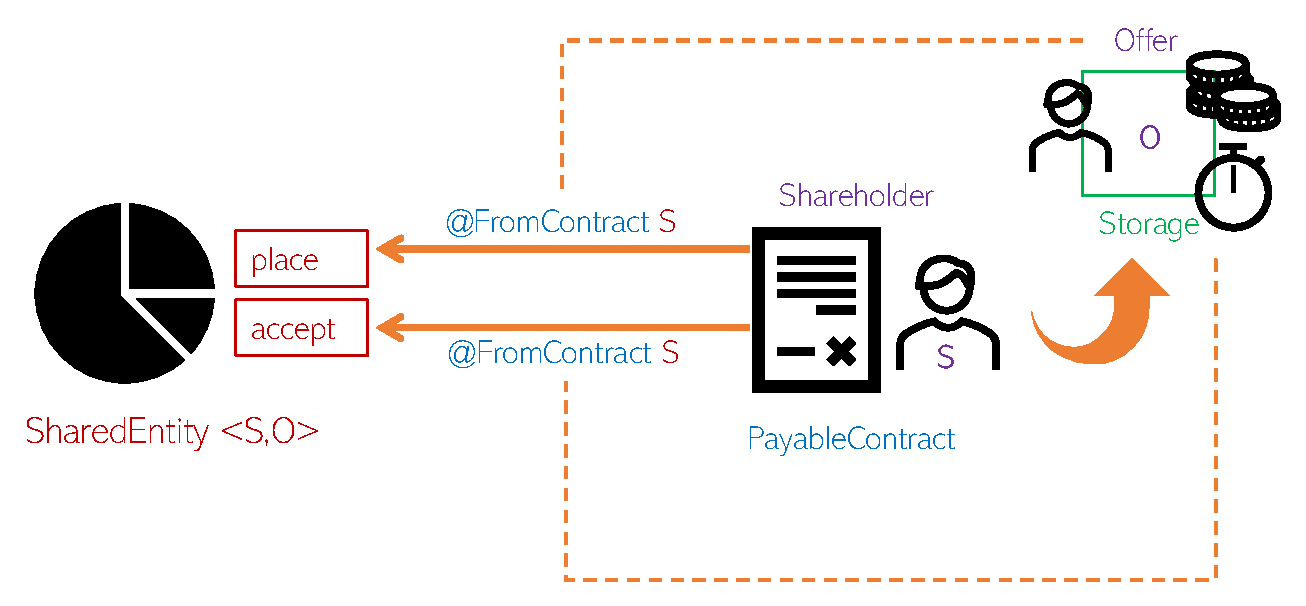
\includegraphics[width=.9\linewidth]{figures/shared_entity}
\caption{Exemplification of a Takamaka shared entity and of its connections with the objects persisted in the blockchain.}
\label{figure.shared_entity}
\end{figure}

As said before, the annotation \<@FromContract> on both \<place> and \<accept> enforces that only
contracts can call these methods.
These callers must be (old or new) shareholders,
hence they must have type \<S>. Therefore, one would like to write
\<@FromContract(S.class)>. Unfortunately, Java does not allow a generic type variable \<S>
in the syntax \<S.class>. Due to this syntactical limitation of Java,
the best we could write in Fig.~\ref{fig:shared_entity} is \<@FromContract(PayableContract.class)>,
which allows \emph{any} \<PayableContract> to call these methods, not just those of type \<S>.
Since the syntax of the language does not support our abstraction, we will have to
program explicit dynamic checks in code, as shown later, and this will be the reason of the
parameter \<buyer> in \<accept>.

Fig.~\ref{fig:simple_shared_entity} shows a portion of our \<SimpleSharedEntity>
implementation of the \<SharedEntity> interface in Fig.~\ref{fig:shared_entity}, that
uses two fields: \<shares> maps each shareholder to the amount of shares the it holds and
\<offers> collects the offers that have been placed.
The constructor initially populates the map \<shares> with the initial shareholder.
Other shareholders can be added later, by buying shares\footnote{In the real code, the class has
  constructors to create shared entities with a \emph{set} of initial shareholders. This paper
  reports a simplification of the actual code.}.
Method \<sharesOf> simply accesses
\<shares>, by using zero as default. Method \<place> requires its \<caller()> to be
the seller identified in the \<offer>. This forbids shareholders to sell shares on behalf of others.
Moreover, this guarantees that the caller has type \<S>, the type of \<offer.seller>.
As it has been said before, this cannot be expressed with the syntax of the language.
Method \<place> further requires the seller to be a shareholder with at least \<offer.sharesOnSale>
shares not yet placed on sale. This forbids to oversell more shares
than one owns. At the end, \<place> adds the \<offer> to the set of \<offers>.
Method \<accept> requires that who calls the method must be \<buyer>. Hence, successful
calls to \<accept> can only pass the same caller for \<buyer>. This is a trick to enforce the
caller to have type \<S>, since the syntax of the language does not allow one to express it,
as we explained before. Then \<accept> requires the \<offer> to exist, to be still ongoing
and to cost no more than the \<amount> of money provided to \<accept>. If that is the case,
the \<offer> is removed from the \<offers>, shares are moved from seller to buyer (code not
shown in Fig.~\ref{fig:simple_shared_entity}) and the seller of the \<offer>
receives the required price \<offer.cost>.

\section{An Attack to the Shared Entities Contract}\label{sec:attack}

Let us state an important property about shared entities:
%
\vspace{2ex}
\begin{mdframed}[leftmargin=10pt,rightmargin=10pt]
  \begin{center}\emph{Consistency of Shareholders}\end{center}
  \noindent
  If \<se> is a {\codesize\texttt{SharedEntity<S,O>}}
  then \<se.getShareholders()> contains only elements of type \<S>.
\end{mdframed}
\vspace{2ex}
%
This property is important since it states that we can trust the type \<S> of
the shareholders: if one creates a \<SharedEntity> and fixes a specific type \<S>
for its shareholders, then only instances of \<S> will actually manage to become shareholders.

It turns out that the \emph{Consistency of Shareholders} property holds
for instances of the class \<SimpleSharedEntity> in Fig.~\ref{fig:simple_shared_entity}.
Namely, that class does not use unchecked casts, hence it is strongly-typed~\cite{NaftalinW06} and
its map \<shares> actually holds values of type \<S> in its domain, only.
For this consistency result, we had to pay the price
of the dummy \<buyer> argument for the method \<accept>
of the shared entities. Without that argument, the
\emph{Consistency of Shareholders} property would not hold, since we could only write
\<addShares((S) caller(), offer.sharesOnSale)> in the implementation of \<accept> in
Fig.~\ref{fig:simple_shared_entity}, with an unchecked cast that makes its code
non-strongly-typed. In that case, also contracts not of type \<S> could call \<accept>
and become shareholders.

There is, however, a problem with the reasoning
in the previous paragraph. Namely, absence of unchecked
operations guarantees strong typing of Java \emph{source} code. But what is installed
and executed in blockchain is the Java bytecode that has been derived from
the compilation of the code in Fig.~\ref{fig:simple_shared_entity}.
Malicious users might install in blockchain some manually crafted bytecode,
not derived from its Java source code compiled together with the source code
in Fig.~\ref{fig:simple_shared_entity}.
That crafted code might
call the methods of \<SimpleSharedEntity>s in order to attack
that contract. In particular,
the signature of method \<accept> declares a parameter \<buyer> of type \<S> at source code level, but
its compilation into Java bytecode declares an erased
parameter \<buyer> of type \<PayableContract> instead.
It follows that an attacker can install in blockchain a snippet of bytecode that calls
\<accept> and passes \emph{any} \<PayableContract>, not only those that are instances of \<S>:
the \emph{Consistency of Shareholders} property is easily violated at bytecode level.

\begin{figure}[t]
  \begin{center}
    \begin{lstlisting}[language=Takamaka]
public class Attacker extends ExternallyOwnedAccount {

  public Validator(String publicKey) {
    super(publicKey);
  }

  @View
  public String id() {
    return /* id of the victim blockchain node, unrelated to publicKey */
  }
}
    \end{lstlisting}
  \end{center}
  \caption{An attacker that exploits the work of a blockchain validator node and fraudolently earns the rewards of that work.}\label{fig:attacker}
\end{figure}

\begin{figure}[b]
\centering
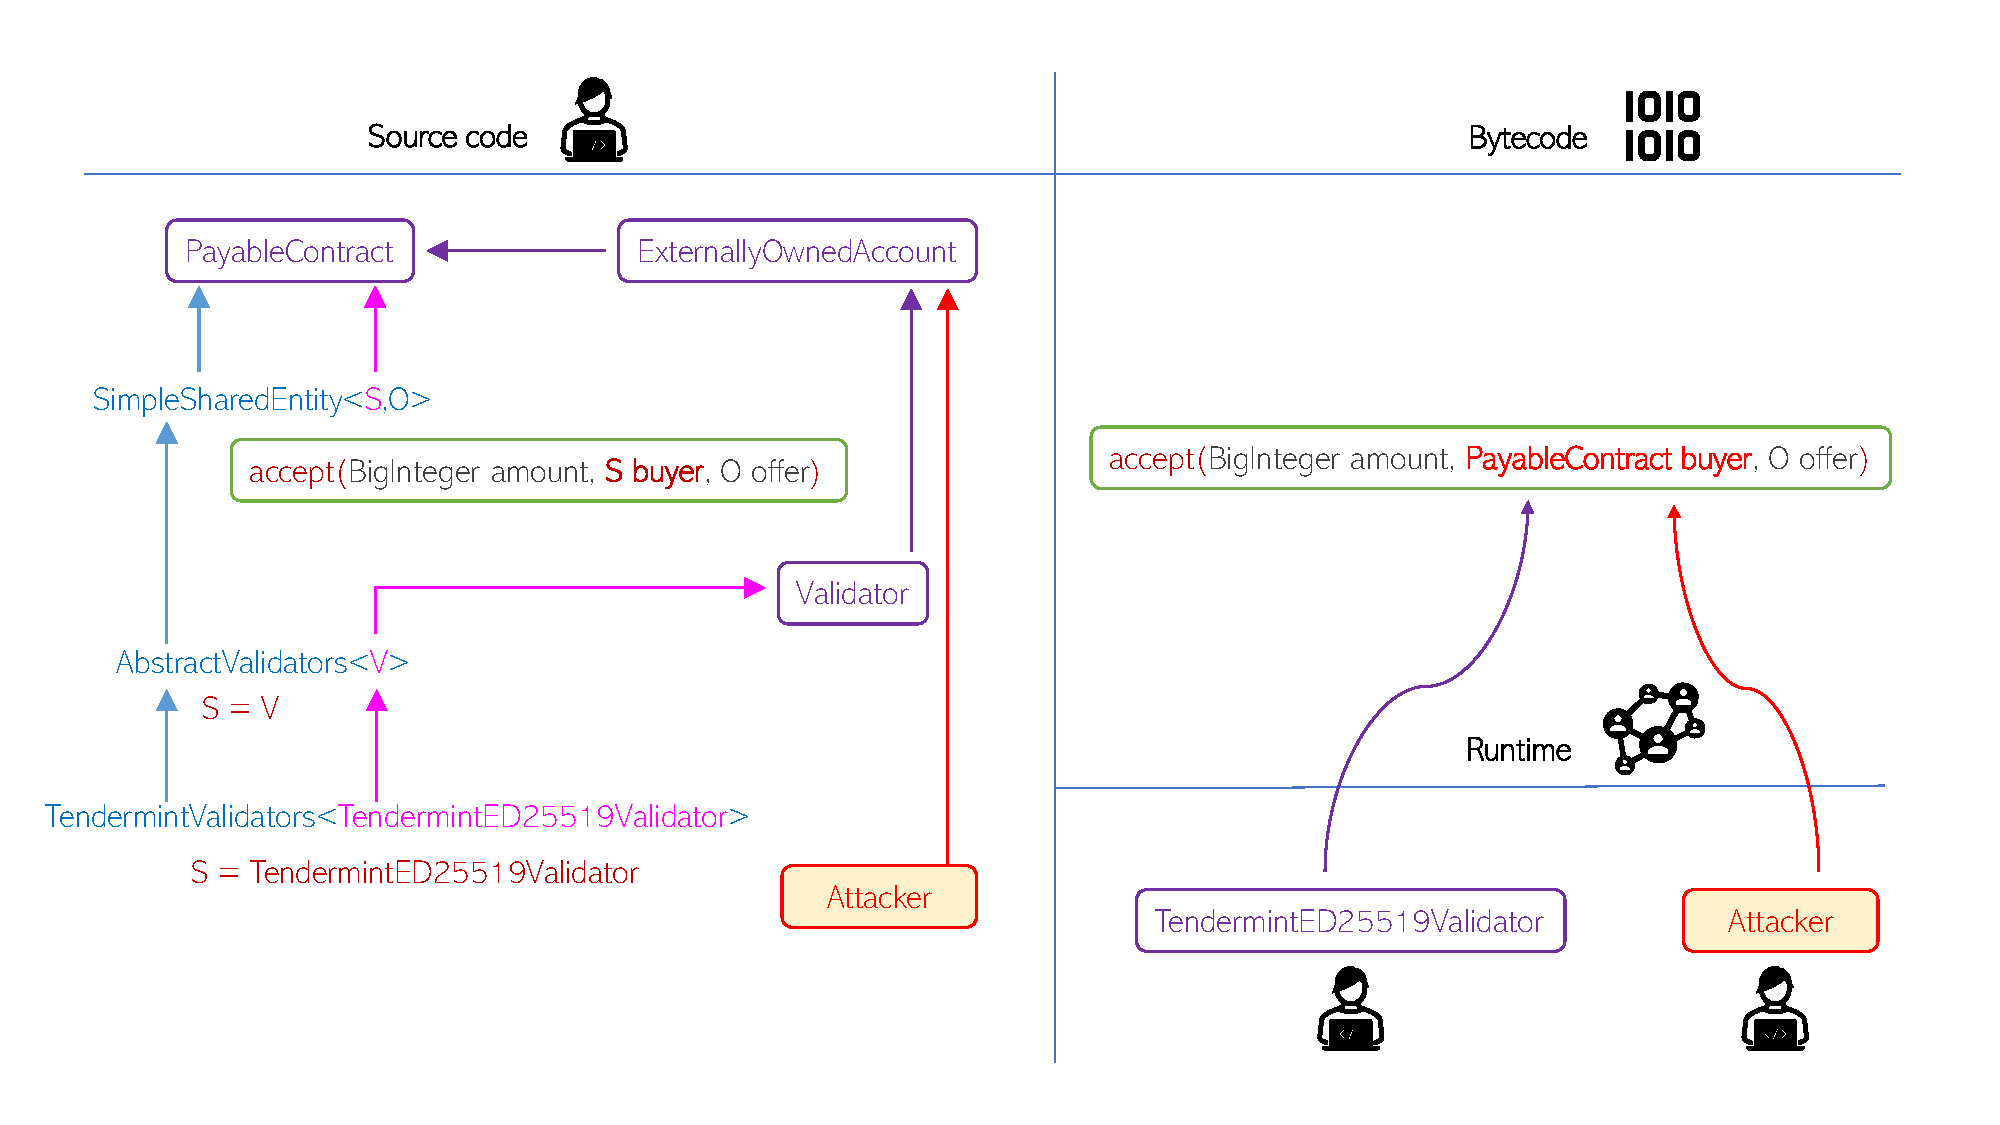
\includegraphics[width=.9\linewidth]{figures/attack}
\caption{Example of possible attack to a smart contract using Java generics.}
\label{figure.attack}
\end{figure}

In particular, it is important that the \emph{Consistency of Shareholders} property holds
for the subclass \<TendermintValidators>: its shareholders
must be \<TendermintED25519Validator>s (as declared in the generic
signature of \<TendermintValidators> in Fig.~\ref{fig:validators}) that enforce a
match between their public key, that identifies who can spend the rewards sent to the validator,
and their Tendermint identifier, that identifies which node of the blockchain
must do the validation work (see how the constructor initializes \<this.id> in
Fig.~\ref{fig:validator}).
If it were possible to add a shareholder of another
type \<Attacker>, the code of \<Attacker> could decouple the node identifier from its
public key (see Fig.~\ref{fig:attacker}):
Tendermint would expect the node (belonging to the \emph{victim}) to do
the validation work while the owner
of the private key of the \<Attacker> could just wait for accrued rewards to spend.
A sort of validator's slavery.
Sec.~\ref{sec:shared_entities} asserted that the \emph{Consistency of Shareholders}
property holds, at source level.
Namely, an \<attacker> (of type \<Attacker>) can only become shareholder
by accepting an ongoing sale \<offer> of shares through a call to
\<tv.accept(offer.cost, attacker, offer)> (Fig.~\ref{fig:simple_shared_entity}).
This is impossible at source level (left part of Fig.~\ref{figure.attack}),
where that call does \emph{not} compile, since \<attacker> has type \<Attacker> that
is not an instance of \<V>, which has been set to \<TendermintED25519Validator>.
But a Hotmoka blockchain contains only the bytecode of \<SimpleSharedEntity>,
where the signature of \<accept> has been erased into
\<accept(BigInteger amount, PayableContract buyer, Offer offer)>
(see Fig.~\ref{figure.java_generics_erasure} and the right part of
Fig.~\ref{figure.attack}).
Hence a blockchain transaction that invokes \<tv.accept(offer.cost, attacker, offer)>
at bytecode level
\emph{does} succeed, since \<attacker> is an externally owned account and all such accounts
are instances of \<PayableContract> (Fig.~\ref{fig:hierarchy-entities}).
That transaction adds \<attacker> to the shareholders of \<tv>,
therefore violating the \emph{Consistency of Shareholders} property and allowing
validator's slavery.

\section{A Solution for Fixing the Compilation of the Contract}\label{sec:fix}

The security issue in Sec.~\ref{sec:attack} is due to the
over-permissive erasure of the signature of method \<accept>,
where the compiler gives \<buyer> the type \<PayableContract>.
Therefore, a solution is to oblige the compiler to generate a more
restrictive signature where, in particular, the parameter \<buyer>
has type \<TendermintED25519Validator>: only that type of accounts
must be accepted for the validators, consequently banning instances of \<Attacker>.

\begin{figure*}[ht]
  \begin{center}
    \begin{lstlisting}[language=Takamaka]
public class TendermintValidators extends AbstractValidators<TendermintED25519Validator> {

  public TendermintValidators(TendermintED25519validator validator, BigInteger power) {
    super(validator, power);
  }

  @Override @FromContract(PayableContract.class) @Payable
  public void accept
    (BigInteger amount, TendermintED25519Validator buyer, Offer<TendermintED25519Validator> offer) {
    super.accept(amount, buyer, offer);
  }
}
    \end{lstlisting}
  \end{center}
  \caption{The fixed code of the shared entity of the validators of a Hotmoka blockchain built over Tendermint.}\label{fig:solution}
\end{figure*}

The fixed code is shown in Fig.~\ref{fig:solution}. The only difference is that method
\<accept> has been redefined to enforce the correct type for \<buyer>
(see that redefined method also in Fig.~\ref{fig:hierarchy-entities}). For the rest, that method
delegates to its implementation inherited from \<AbstractValidators>, through a call
to \<super.accept>.
It is important to investigate which is the Java bytecode generated from
the code in Fig.~\ref{fig:solution}. Since Java bytecode does not allow one to redefine a method
and modify its argument types, the compiled bytecode actually contains \emph{two}
\<accept> methods, as follows:

\begin{lstlisting}[language=JavaBytecode]
public class TendermintValidators extends AbstractValidators {
  ...
  
  public void accept(BigInteger,TendermintED25519Validator,Offer)
   aload_0
   aload_1
   aload_2
   aload_3
   invokespecial AbstractValidators.accept
       (BigInteger,PayableContract,Offer)
   return

  // synthetic bridge method
  public void accept(BigInteger,PayableContract,Offer)
   aload_0
   aload_1
   aload_2
   checkcast TendermintED25519Validator
   aload_3
   invokevirtual accept
       (BigInteger,
        TendermintED25519Validator,
        Offer)
   return
}
\end{lstlisting}

\noindent
The first \<accept> method above is the compilation of that from Fig.~\ref{fig:solution}:
it delegates to the \<accept> method of the superclass \<AbstractValidators>. The second
\<accept> method above is a \emph{bridge method} that the compiler generates in order to guarantee
that all calls to the erased signature \<accept(BigInteger,PayableContract,Offer)> actually
get forwarded to the first, redefined \<accept>. It casts its \<buyer> argument
into \<TendermintED25519Validator> and calls the first \<accept>. This
bridge method and its checked cast guarantee that only \<TendermintED25519Validator>s
can become validators. As shown in Fig.~\ref{figure.solution},
an instance of \<Attacker> (Fig.~\ref{fig:attacker})
cannot be passed to the first \<accept> (type mismatch) and makes the second \<accept>
fail with a class cast exception. The \emph{Consistency of Shareholders} holds
for instances of \<TendermintValidators> now and the attack in Sec.~\ref{sec:attack} cannot occur
anymore.

The solution of redefining method \<accept> can be seen as a limited form of heterogeneous
compilation of generics, restricted to a specific method and forced manually.
It is interesting to consider which methods
would need that redefinition, in general. They are those that have a parameter of a generic type
that is restricted in a subclass. For instance, method \<accept> in
Fig.~\ref{fig:shared_entity} has parameters \<buyer> and \<offer> of generic type
\<S> and \<O>, respectively. The subclass in Fig.~\ref{fig:validators} restricts
\<S> to be a \<TendermintED25519Validator> and \<O> to be
an {\codesize\texttt{Offer<TendermintED25519Validator>}}. Hence we must redefine
\<accept> in the subclass with the more specific types for the \<buyer> and \<offer>
parameters. In the future, a compiler might perform this automatically or a static analysis
tool might issue a warning when such redefinition is needed. Currently, however, that is
left to the programmer of the smart contracts, who might overlook the problem
and give rise to security issues, as shown in Sec.~\ref{sec:attack}.

\begin{figure*}[ht]
\centering
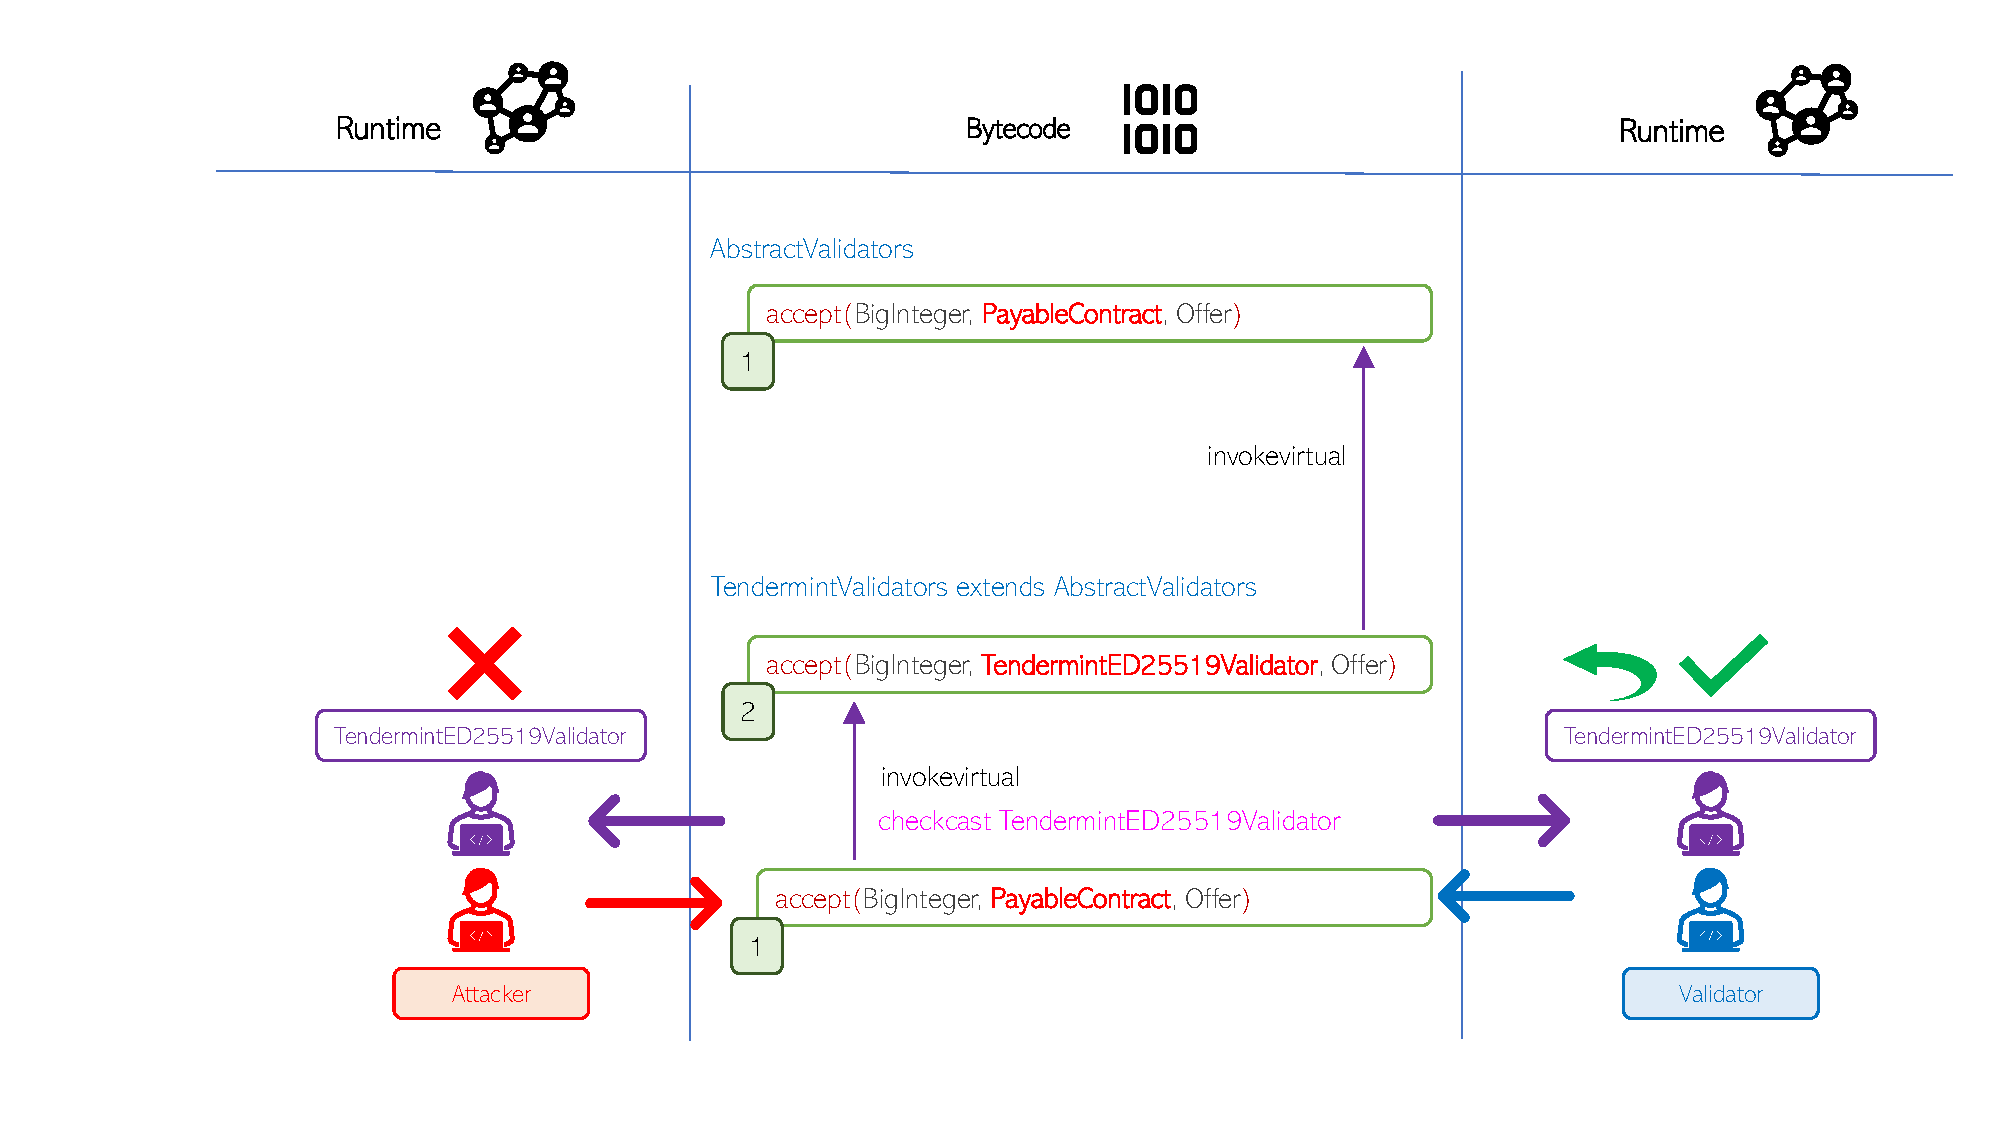
\includegraphics[width=0.9\linewidth]{figures/solution}
\caption{Example of how the proposed solution works at run time when the \<accept> method is called by a \<Validator> or an \<Attacker>.}
\label{figure.solution}
\end{figure*}


\section{Related Work}\label{sec:related_work}

% \todo{Forse questa parte va spostata.}
% 
% 
% \textbf{Compilation of generics --}
% Generics is a way for writing code parametrized by type, in other words 
% a same piece of code can be written by using a type placehorder 
% (a \emph{type parameter}) and then instantiated for specific,
% concrete types. There exists two common ways to implement generics in 
% a programming language, that are often described in literature~\cite{generics_categories}
%  as \emph{heterogeneous} and \emph{homogeneous}. In the heterogeneous 
% approach the code is specialized for each instance
% of the generic parameter; this is the approach adopted by C++ \emph{templates}.
% Conversely, the homogeneous approach is the one provided by Java and .Net; 
% in this case, only one instance of the code is maintained and shared by 
% all generic instances.
% This implementation is based on the type \emph{erasure} mechanism, where the 
% generic parameter is replaced by the upwards bound of each instance, most 
% often \<Object>.
% Even if the heterogeneous approach is the safest, it is rarely applied in particular
% in resource-constrained applications, because the code size may dramatically increase
% as some code is duplicated~\cite{generics_embedded_systems}. For code in blockchain,
% the heterogeneous approach obliges one to reinstall all instantiations of the 
% generic code, with extra costs of gas.
% Conversely, the homogeneous approach ensures a smaller consumption
% of resources but can lead to the problems described in this paper. \\
% 
% \textbf{Smart contracts vulnerabilities --}

It has been estimated that, on average, software developers make from 100 to 150 errors
for every thousand lines of code~\cite{software_engineering}.
In 2002, the National Institute of Standards and Technology (NIST) estimates that the economic
costs of faulty software in the US is about tens of billions of dollars per year and represent
approximately just under 1 percent of the Nation's gross domestic product.
The effects induced by errors in software development are even worse when such pieces of software
are smart contracts. Indeed, it is usually impossible to change a smart contract once
it has been deployed, the immutability being one of its main characteristics, so that
errors are treated as intended behaviours. Moreover, smart contracts often store and
manage critical data such as money, digital assets and identities. For this reason, smart contracts
vulnerabilities and correctness are becoming important in literature\,\cite{smart_contracts_verification}. Possible solutions can be
classified into three main categories: (i) static analysis of EVM bytecode,
(ii) automatic rectification of EVM bytecode and (iii) development of new languages
for smart contracts.

Given the plurality of languages currently available for the design of smart contracts,
static analysis is usually performed directly on the Ethereum bytecode, in order to make
the solution general enough and promote its adoption. At this regards, SafeVM~\cite{safevm}
is a verification tool for Ethereum smart contracts that works on bytecode and exploits
the state-of-the-art verification engines already available for C programs.
The basic idea is to take as input a smart contract in compiled bytecode, that
can possibly contain some \<assert> or \<require> annotations, decompile it and convert it
into a C program with \<ERROR> annotations. This C program can be verified by using
existing verification tools.
%
In~\cite{hol_smart_constracts}, the authors propose a verification tool for Ethereum
smart contracts based on the use of the existing Isabelle/HOL tool, together with the
specification of a formal logic for Ethereum bytecode. More specifically, the desired properties
of the contracts are stated in pre/postcondition style, while the verification
is done by recursively structuring contracts as a set of basic blocks
down to the level of instructions.
%
Another tool for the analysis of Ethereum bytecode is EthIR~\cite{ethir}. This open-source tool
allows the precise decompilation into a high-level, rule-based representation. Given such
representation, properties can be inferred through available state-of-the-art analysis tools
for high-level languages. More specifically, EthIR relies on an extension of Oyente,
a tool that generates code control-flow graphs in order to derive
a rule-based representation of the bytecode.
%
Considering the specific case of the Java language,
formal techniques for static analysis can be built, for instance, over
the Featherweight Java calculus~\cite{IgarashiPW01}, or by abstract
interpretation~\cite{Spoto16}. Currently, however, we are not aware
of formal verifications for generics, at bytecode level.

Relatively to the automatic certification of smart contracts,
Solythesis~\cite{solythesis_solidity_validation} is a compilation tool for smart contracts
that provides an expressive language for specifying desired safety invariants.
Given a smart contract and a set of user defined invariants,
it is able to produce a new enriched contract that will reject all transactions
violating the invariants.
%
Another solutions, based on bytecode rewriting, is presented in~\cite{bytecode_rewriting},
where the authors propose the enforcement of security policies through the enhancement of bytecode.
More specifically, the disassembled bytecode is instrumented through new security guard code
that enforces the desired policy. Their initial efforts are mainly focused on the verification
of arithmetic operations, such as the prevention of overflows. In the future, they plan to focus on
verifying memory access operations.
%
SMARTSHIELD~\cite{smartshield} is another tool for automatically
rectifying bytecode with the aim to fix three typical security bugs in smart contracts:
(i) state changes after external calls, (ii) missing checks for out-of-bound arithmetic operations,
and (iii) missing checks for failing external calls. More specifically, given an identified issue,
the tool performs a semantic-preserving code transformation to ensure that only the insecure code
patterns are revised, eventually sending the rectification suggestions back to the developers
when the eventual fixes can lead to side effects. The tool not only guarantees that the rectified
contracts are immune to certain attacks but also that they are gas-friendly.
Indeed, it adopts heuristics to optimize gas consumption. 

%Given the plurality of verification tools that have been developed for indentifying security bugs
%in smart contracts, a unified and standard approach for evaluating their accuracy and performances
%have been developed in~\cite{effectiveness_analysis_tools}. This automated and systematic approach,
%called SolidiFI, consists in injecting bugs into all potential locations in a smart contract,
%in order to introduce different kinds of vulnerabilities, and then using several static analysis
%tools to identify which bugs each of them is able to detect.

Finally, as regards to the definition of new programming languages for safe smart contracs,
Scilla~\cite{scilla} has been tailored by taking System~F as a foundational calculus.
It is able to provide strong safety guarantees by means of type soundness.
Thanks to its minimalistic nature, it has been possible to define also a generic and extensible
framework for lightweight verification of smart contracts by means of user-defined domain-specific
analyses. The type variables of the functional foundational calculus can be seen as
generic types. We do not know how they are compiled and if the strong typing guarantee of the
source code extends to the compiled code as well. Scilla contracts are developed with
the Neo Savant online IDE. Currently, neither Neo Savant IDE nor the block explorer
allow one to inspect the compiled bytecode, in order to undertsnad how generic types are compiled.


\section{Conclusion}\label{sec:conclusion} 

This paper has shown that generics are useful in the definition
of smart contracts and can simplify the development of rather complex
code such as that for shared entities, and support code reuse, for
instance to implement the validators set of a blockchain network.
However, this paper has shown that generic types
introduce risks of security as well.
Namely, many
programming languages, including Java, erase them at compile time
into types that might be too permissive for low-level calls, such as
those that are started by blockchain transactions. Note that the use of a programming
language without generics is not the solution: Solidity has no generics
and consequently erases \emph{all} reference types into \<address>.
That is the worst possible erasure.

The solution in this paper has been to redefine the methods that have an argument
of generic type, in such a way to call their superclass
(see the case of \<accept> in Fig.~\ref{fig:solution}). This fixes the security risk,
but cannot be regarded as the definite solution to the problem. It is just a trick that
works because it forces the compiler to generate some specific kind of bytecode.
A \emph{smarter} compiler might recognize the redefined \<accept> as
\emph{useless} and just remove it. This would recreate the issue that
has been just solved. That is, the solution in this paper works only for the way
compilers compile \emph{today}.

With hindsight, it is questionable to have implemented generics by erasure
and code instrumentation (bridge methods). If generics would be present
and checked at bytecode level, the attack in Sec.~\ref{sec:attack} would just
be impossible. Currently, generics can only exist as bytecode annotations
that are not mandatory and are ignored by the Java virtual machine
that runs the bytecode. The same consideration might be applied beyond
generics: many features of modern programming
languages have no direct low-level
counterpart but are implemented via instrumentation. Examples are
inner classes and closures (lambda expressions). This is fine at source level, but allows
low-level calls to easily circumvent
the encapsulation guarantees of the language. When embedded in a permissionless
blockchain, such features become dangerous attack surfaces. This paper has shown
the attack surface due to redefinition of methods with a generic parameter.
But another example is the use of instrumented methods to allow access to
private state from inner classes: since inner classes are compiled into distinct
bytecode classes, the compiler adds non-private accessors to the
private state. These accessors cannot be used
at source level, but can be called at bytecode level to gain access to private state.
This paper does not provide a solution to this other issue, but this further example
makes it clear that the attack surface is larger than what described here.

\section{Compliance with Ethical Standards}

This work was partially supported by ``Progetto di Eccellenza''
of the Computer Science Department of University of Verona, Italy.

The authors declare that they have no conflicts of interest.

This article does not contain any studies involving animals performed by any of the authors.

This article does not contain any studies involving human participants performed by any of the authors

\section{Data Availability Statements}

The source code is freely available at \url{https://github.com/Hotmoka/hotmoka/tree/master/io-takamaka-code}



\bibliographystyle{plain}
\bibliography{biblio}

\end{document}
